\section{Implementierung des Senders}
\label{sec:imp_des_transmitters}
Abb.~\ref{fig:transmitter} zeigt den funktionsfähigen Sender im GRC. Der Sender transportiert zwei Audio Kanäle im MSC, wobei der obere Kanal einen DAB+ Audio Stream (MPEG4 und Reed Solomon Encoder) und der untere Kanal einen DAB Audio Stream (MPEG 2 Encoder) transportiert. Jeder Block in der grafischen Ansicht entspricht einer eigenen C++ Klasse, wobei die Kanalcodierer des FIC und MSC, sowie der OFDM Modulator hierarchische Blöcke darstellen, also mehrere C++ Blöcke in sich zusammenfassen. Die Struktur der Blöcke als einzelne Funktionseinheiten ist von der Aufteilung dem DAB Standard nachempfunden. Bei der Implementierung wurde darauf geachtet, möglichst viel Funktionalität in eine Klasse zu integrieren ohne dabei an Flexibilität der einzelnen Blöcke einzusparen.

\begin{figure}[ht]
\centering
  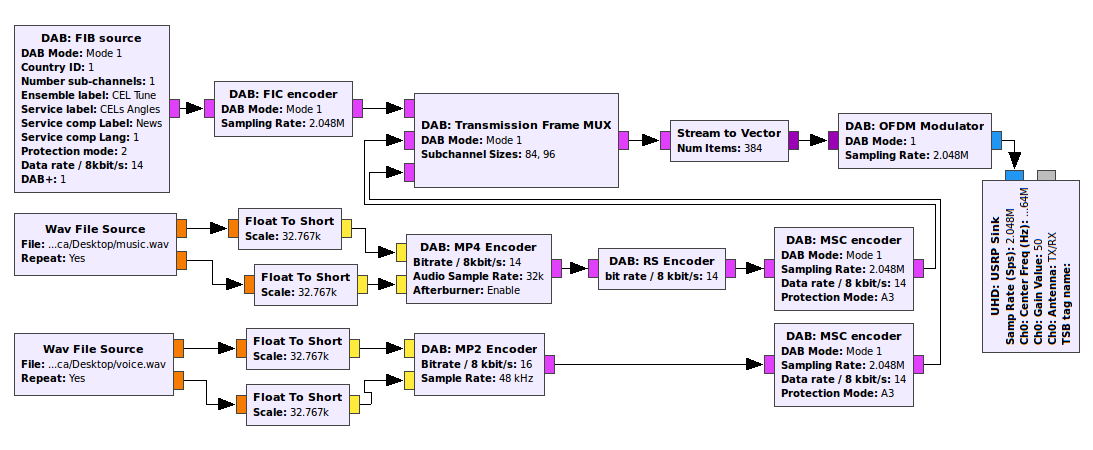
\includegraphics[width=\textwidth]{figures/GRC_transmitter.png}
	\caption{DAB/DAB+ Sender im GRC}
	\label{fig:transmitter}
\end{figure}

\subsection{FIB Quelle}
Die FIB Quelle produziert standardkonforme FIBs für den FIC. Die \ac{MCI} und \ac{SI} werden der Klasse dabei als Argumente übergeben. Die folgenden Informationen werden gesendet:
\begin{itemize}
\item Ensemble Informationen: Länder ID, Ensemble ID, CIF Zähler
\item Radiosender-Organisation: Länder ID, Anzahl der Radiosender, Senderbeschreibung
\item Radiosender-Komponenten: Kanal ID, Audio Typ, Primär-/Sekundärsender
\item Kanal Organistaion: Kanal ID, Start und Länge (in CUs), Protection Mode
\item Service Information (SI): Namensbeschriftung für das Ensemble und jeden Radiosender und deren Sprache
\end{itemize}
Diese FIBs umfassen bei weitem nicht das ganze Spektrum der möglichen Metadaten. Sie sind aber ausreichend um dem Empfänger die nötigen MCI für die Decodierung und dem Nutzer die Informationen zur Identifikation der Programme zur Verfügung zu stellen. Weil die MCI eine weit höhere Wichtigkeit als die SI einnimmt, wird sie periodisch mit jedem CIF gesendet. Die Größe der gesamten MCI hängt von der Anzahl der verwendeten Services und Service Komponenten ab. Bei einer Begrenzung auf maximal 7 Radiosender mit je einem Kanal kann die Information in den ersten zwei FIBs gespeichert werden. Im dritten FIB wird dann die SI geschrieben.

% FIB Aufteilung
\begin{figure}[htb]
\begin{center}
\begin{tabular}{|c|c|c|c|c|}
  \hline
  \multicolumn{3}{ |c| }{\textbf{FIB 1}} & \textbf{FIB 2} & \textbf{FIB 3} \\
  \hline
  Ensemble & Radiosender & Komponente & Kanal & Service \\
  Information & Information & Information & Organisation & Information \\
  \hline
\end{tabular}
\end{center}
\caption{FIC Sendestruktur}
\label{tab:fic_struct}
\end{figure}

Da eine Namensbeschriftung mit 16 Buchstaben ein FIB schon nahezu füllt, werden die einzelnen Labels nacheinander jeweils im dritten FIB verschickt. Dies ist nicht problematisch, da die Namen der Radiosender im Regelfall über die Zeit konstant bleiben und durch eine CIF Rate von $\frac{1}{24 ms} > 41 \: \text{CIFs}/s$ trotzdem jedes Label mehrmals pro Sekunde gesendet wird.

\subsection{FIC Encoder}
\label{sec:fic_encoder}
Der FIC Encoder ist in einem hierarchischen Block implementiert, dessen beinhaltete C++ Blöcke in Abb.~\ref{fig:fic_encoder} dargestellt sind. Er fasst die gesamte Kanalcodierungskette aus Kap.~\ref{sec:FIC} zusammen. Während für die CRC Berechnung und die Faltungscodierung eine jeweilige Klasse implementiert wurde, besteht die Energieverwischung, wie in Gl.~\ref{eq:energy_dispersal} beschrieben, lediglich aus einer XOR Verknüpfung des Bitstreams mit der PRBS Folge, was mit vorhanden GNU Radio Blöcken realisierbar ist.

\begin{figure}[ht]
\centering
  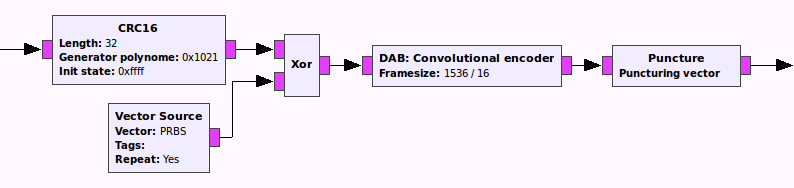
\includegraphics[width=\textwidth]{figures/FIC_encoder.png}
	\caption{Kanalcodierung im hierarchischen Block des FIC Encoders}
	\label{fig:fic_encoder}
\end{figure}

\subsection{Audio Quellen und Encoder}
Die Eingangsdaten der Audioencoder sind 16 bit \ac{PCM} Samples. Um Audio für den Stream zur Verfügung zu stellen gibt es verschiedene Möglichkeiten. Entweder werden Audiosamples über eine Binärdatei als Rohdatenquelle genutzt. Eine andere Möglichkeit bietet der \glqq WAV File Source\grqq{} Block von GNU Radio, der aus dem populären \glqq WAVE\grqq{} Audioformat die Rohdaten extrahiert und somit auch eine PCM Quelle darstellt. Eine letzte Möglichkeit ist die direkte Generation von PCM Samples über die lokale Soundkarte. Alle drei Möglichkeiten resultieren letztendlich in einem Stream mit 16 bit Gleitkommawerten, dessen Samplingrate der Audiorate entspricht. Weil die implementierten Audiocodecs auf Integerebene arbeiten, wird der Stream vor der Audioencodierung auf den neuen Wertebereich abgebildet (siehe Abb.~\ref{fig:transmitter}).

\subsubsection{MPEG 1/2 Audio Layer II Encoder (DAB)}
Der MPEG 2 Encoder Block verwendet einen Patch der frei verfügbare MPEG2 Encoder Bibliothek \textit{TooLAME}. Der Patch stammt vom \textit{ODR mmbTools} Projekt \cite{repo:odr_audioenc} und ist speziell auf DAB Audio Encoding angepasst. Der Code wurde in einen GNU Radio Block integriert um ihn in einen Flowgraph einbauen zu können. Die Funktionalität des Encoder Blocks kann mit einem Loopback-Test verifiziert werden, indem der encodierte Stream mit einem Audio-Player erfolgreich und fehlerfrei decodiert und abgespielt wird.

\subsubsection{MPEG 4 HE-AACv2 (DAB$+$)}
Der MPEG 4 Encoder basiert auf einem Patch der \textit{FDK-AAC Codec Bibliothek für Android der Fraunhofer-Gesellschaft zur Förderung der angewandten Forschung e.V.} \cite{repo:fdk-aac}. Die Bibliothek untersützt eine Reihe von AOTs (Audio Optimization Tools) welche die Audiokompression nach unterschiedlichen Paramtern optimieren. Es stehen die folgenden AOTs zur Verfügung:
\begin{itemize}
\item AAC-LC: Geringe Komplexität ($1,5$ bits/Sample) für minimales Codierungsdelay
\item HE-AAC Dualband SBR: Hohe Effizienz ($0,625$ bits/Sample) durch Spektralbandreplikation.
\item HE-AAC v2 PS: Zusätzlich mit parametrisiertem Stereo ($0,5$ bits/Sample)
\end{itemize}
Der DAB+ Standard enthält neben der neuen Audiokompression mit HE-AAC v2 eine zusätzliche Fehlererkennung und Fehlerkorrektur. Jeweils 5 Logische DAB Frames bilden ein sog. DAB+ Superframe, das den Inhalt eines MPEG 4 Frames aufnimmt. Der Header dieses Frames wird mit einem CRC Wort, dem sog. Firecode, versehen. Die Fehlerkorrekturfähigkeit wird durch Reed-Solomon Codes RS(120, 110, t=5) erreicht. Ein Superframe wird blockweise um jeweils 10 Codebytes pro 110 Datenbytes ergänzt. Der Reed-Solomon Code ist durch diese eingeführte Redundanz empfängerseitig in der Lage maximal 5 Fehler pro 120 Byte Block zu erkennen und zu korrigieren.\\
Um den MPEG 4 Encoder Block nicht zu sehr auf DAB+ zu spezialisieren, wurde der Firecode sowie der Reed-Solomon Encoder jeweils in einem separaten Block implementiert.

\subsection{MSC Encoder}
Der MSC Encoder entpricht von Aufbau und Struktur dem FIC Encoder Block aus Kapitel \ref{sec:fic_encoder}, wobei er keinen CRC Block besitzt und um eine zusätzliche Klasse für das Zeitinterleaving ergänzt ist.\\
Die durch das Zeit-Interleaving eingeführte Verzögerung um bis zu 15 Logische Frames (siehe Abschn.~\ref{sec:time_interleaving_std}) stellt die Implementierung des Zeit-Interleaving Blocks vor Herausforderungen. Zum einen benötigt der Block ein Gedächtnis von 15 Logischen Frames. Ein dynamisches Speichern dieser Frames in Objekte der Klasse kostet viel Rechenleistung und ist daher unbedingt zu vermeiden um das System echtzeitfähig zu halten. Anstelle dessen, werden die jeweils letzten 15 Frames nach deren eigentlichen Verarbeitung nicht aus dem Eingangsbuffer entfernt, sondern der Pointer des Eingangsbuffers wird um 15 Frames verschoben. Der Eingangsbuffer ist damit zu jeder Zeit um 15 Frames größer, es müssen aber keine zusätzlichen Kopieroperationen durchgeführt werden.\\
Zum anderen stellt der Beginn des Streams ein Problem für den Algorithmus dar. An dieser Stelle liegt dem Zeit-Iterleaver noch keine Historie vor, sodass er keine Möglichkeit hat, mit dem Interleaving zu beginnen. Aus diesem Grund wird die Historie des Blocks initial mit 15 Frames gefüllt, die Nullen enthalten.

\subsection{Multiplexer}
Der Multiplexer Block hat prinzipiell die Aufgabe eines Parallel-Seriell Wandlers. Er besitzt einen Eingang für den FIC und eine variable Anzahl an Eingängen für den MSC und setzt alle Kanäle zu einem Sendesignale nach der Struktur aus Kapitel \ref{sec:transmission_frame} zusammen. Die Position der jeweiligen Audiostreams im CIF werden dabei über die selbe MCI bestimmt, die in den FIBs des FIC desselben Sendeframes stehen. Die Synchronisationssymbole $z_{0,k}\, \text{und}\, z_{1,k}$ sind an dieser Stelle noch nicht vorhanden und werden dem Sendeframe im OFDM Modulator hinzugefügt.

\subsection{OFDM Modulator}
Der OFDM Modulator Block ist ein hierarchischer Block mit vielen Unterklassen. Jede Klasse führt dabei einen der in \ref{sec:ofdm_mod} beschriebenen Schritte zur Modulation durch.

\subsubsection{QPSK Mapping}
Der QPSK Mapper bildet 1 Byte auf 4 komplexe QPSK Symbole ab. Da wie in \ref{sec:qpsk} beschrieben zuerst die Realteile und anschließend die Imaginärteile eines kompletten OFDM Symbols übertragen werden, kann der QPSK Mapper nicht Byte für Byte arbeiten, also jedes Byte direkt auf 4 QPSK Symbole abbilden. Deshalb arbeitet der Mapper auf Vektorbasis der Länge $1536/4$ bits am Eingang, bzw. $1536$ bits am Ausgang. Dies umfasst genau die Länge eines OFDM Symbols.

\subsubsection{Einfügen des Phasenreferenzsymbols}
Das Phasenreferenzsymbol wird schon als ein um $\pi/4$ gedrehtes QPSK Symbol generiert. Daher wird es erst nach der QPSK Modulation der Datensymbole an das Sendeframe angehängt. Das Phasenreferenzsymbol ist bei jedem Sendeframe gleich und kann deshalb im Konstruktor einmalig generiert werden um bei Laufzeit nur noch in den Buffer kopiert zu werden.

\subsubsection{Differentielle Modulation}
Die Differentielle Modulation stellt eine komplexe Multiplikation jedes Symbols mit dessen Vorgänger dar (siehe~\ref{sec:diff_mod}). Auch hier wird auf Vektorbasis gearbeitet.

\subsubsection{Frequenzinterleaving}
Vor der OFDM Modulation müssen die 1536 D-QPSK Symbole auf die IFFT Länge von 2048 gebracht werden. Dazu werden symmetrisch am Anfang und Ende des Vektors jeweils 256 Nullelemente eingefügt.\\
Das anschließende Vertauschen der OFDM Unterträger folgt der Regel
\begin{equation}
\begin{aligned}
\Pi(i) &= (13\, \Pi(i-1) + 511)\; \text{mod}\; 2048 \quad \text{mit} \quad i \in [0,1536)\\
\text{und} \quad \Pi (0) &= 0
\end{aligned}
\end{equation}
wobei $\Pi(i)$ die Permutation ist, die sich aus deren Vorgänger $\Pi(i-1)$ ergibt. Da diese Vertauschungsregel bei jedem Symbol die selbe ist, wird im Konstruktor des Frequenzinterleaving Blocks einmalig eine Umsetzungstabelle für die $T_S=2048$ Permutationen generiert. Dadurch benötigt der Block zur Laufzeit weniger Rechenzeit.

\subsubsection{\ac{IFFT}}
Die OFDM Operation kann nach~\ref{sec:ofdm} als \ac{IDFT} durchgeführt werden. Wegen $2048 = 2^{11}$ kann die IDFT als eine deutlich schnellere IFFT realisert werden. Eine IFFT Implementierung ist in dem GNU Radio Modul \glqq gr-fft\grqq{} vorhanden \cite{repo:gr-fft} und wird verwendet.

\subsubsection{Einfügen des Cyclic Prefixes}
Nach der IFFT liegt das Sendesignal nun im Zeitbereich vor. Das Einfügen des Cyclic Prefixes (CPs) entspricht dem Kopieren vom Ende jedes Symbols an den Anfang. Da CPs eine breite Anwendung in der Nachrichtentechnik haben, existiert in GNU Radio schon ein Block mit dieser Funktionalität, der nur noch mit der passenden Symbollänge $T_S = 2048$ Samples und der Länge des Cyclic Prefixes $T_G = 504$ Samples initialisiert wird.

\subsubsection{Einfügen des Nullsymbols}
Als letzter Schritt in der Sendekette erfolgt das Einfügen des Nullsymbols. Dabei werden $T_{NULL}=2656$ Samples mit dem Wert $0+0j$ zwischen zwei Sendeframes geschrieben.

\subsubsection{}
Das Basisbandsignal ist nun bereit um hochgemischt und anschließend gesendet zu werden. Beide Schritte sind in dem GNU Radio Block \textit{USRP Sink} vereint, der die Schnittstelle zwischen Software und Hardware bildet. Alternativ lässt sich das Basisbandsignal natürlich auch als I/Q Daten in einer Binärdatei speichern.